% Компіляція: lualatex -shell-escape main.tex
\documentclass[12pt,a4paper]{article}
\usepackage{fontspec,polyglossia}\setdefaultlanguage{ukrainian}\setmainfont{NewComputerModern10}\setmonofont{Noto Sans Mono}[Scale=.82]
\usepackage{amsmath,booktabs,caption,enumitem,float,fvextra,geometry,graphicx,hyperref,microtype,tikz,titlesec}
\usetikzlibrary{arrows.meta,positioning}
\geometry{left=2cm,right=2cm,top=2cm,bottom=2cm}\setlength{\parindent}{1.25cm}\setlength{\parskip}{0pt}\linespread{1.0}\setlength{\emergencystretch}{3em}
\captionsetup{font=small,labelfont=bf,labelsep=endash}
\titleformat{\section}{\normalfont\fontsize{14}{16}\selectfont\bfseries\centering}{\thesection.}{.6em}{}
\titleformat{\subsection}{\normalfont\fontsize{12}{14}\selectfont\bfseries\centering}{\thesubsection.}{.6em}{}
\begin{document}\pagenumbering{gobble}
\begin{titlepage}
\begin{center}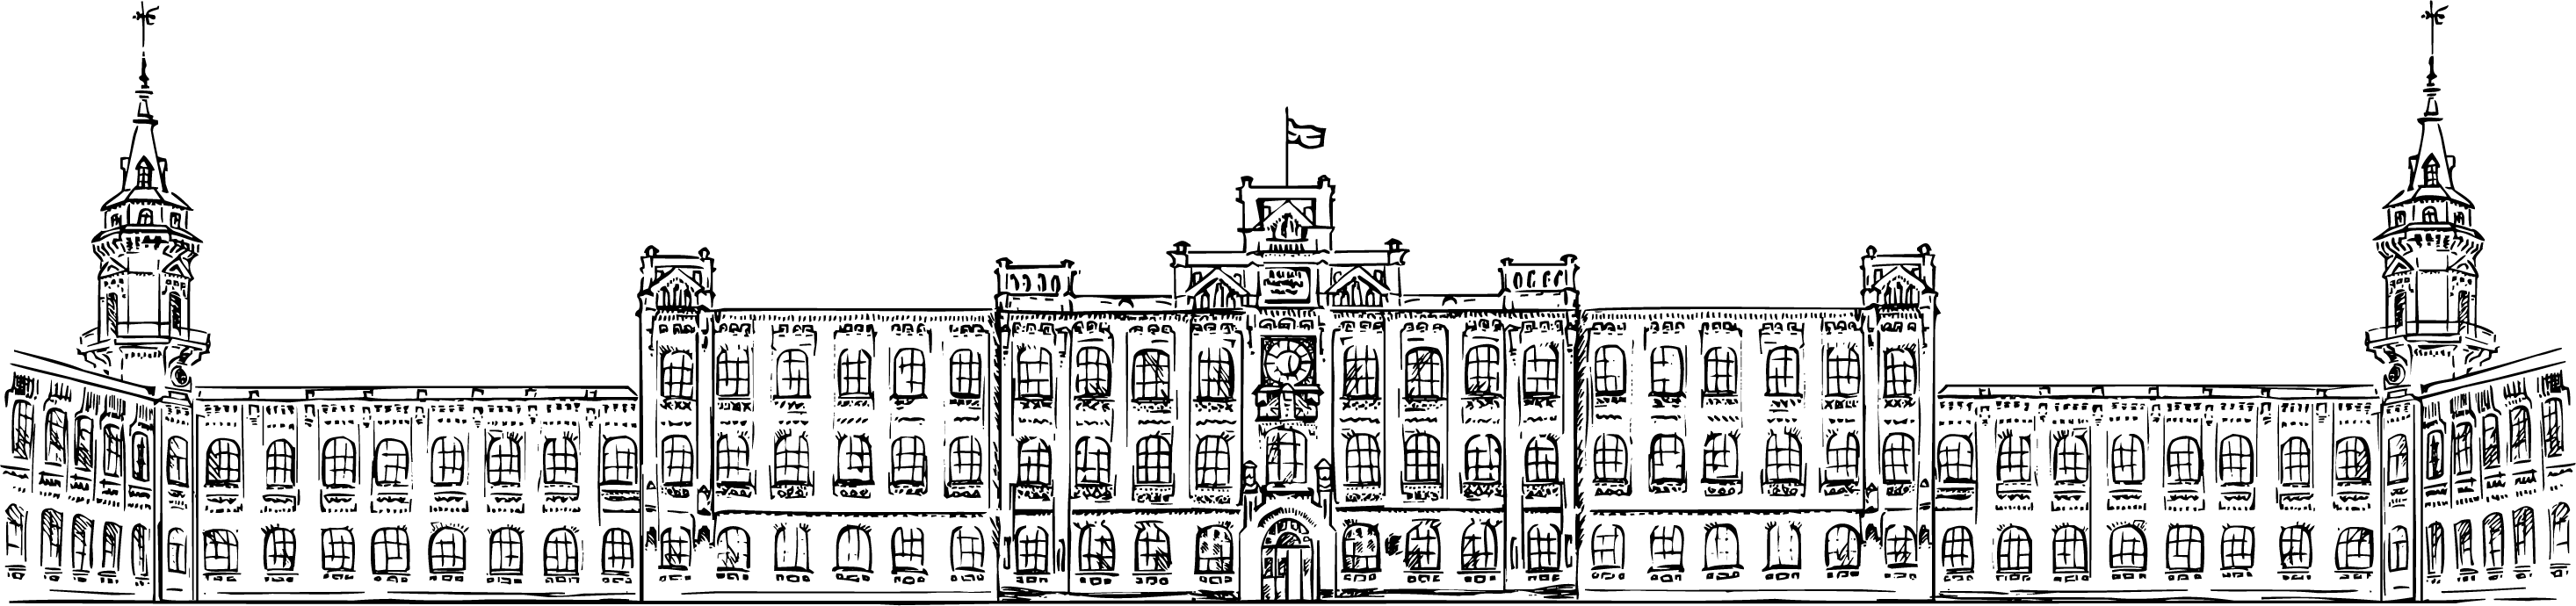
\includegraphics[width=.7\textwidth]{../../../../../../templates/letterhead.png}\end{center}
\begin{center}\large Національний технічний університет України\\«Київський політехнічний інститут імені Ігоря Сікорського»\\[1em]Факультет інформатики та обчислювальної техніки\\Кафедра обчислювальної техніки\end{center}
\vfill\begin{center}\textbf{\LARGE Технології Computer Vision}\\[2em]\textbf{\Large Лабораторна робота №6}\\[.7em]«Технології ідентифікації в Computer Vision»\end{center}
\vfill\begin{flushright}\begin{minipage}{.48\textwidth}Виконав: студент 3 курсу ФІОТ,\\групи ІО-41\\\textit{Давидчук А. М.}\\Залікова книжка № 4106\\[1em]Перевірив: \textit{Баран Д. Р.}\end{minipage}\end{flushright}
\vfill\begin{center}Київ --- 2026\end{center}\end{titlepage}
\pagenumbering{arabic}

\section{Тема та мета роботи}
\noindent\textbf{Тема:} технології ідентифікації об'єктів у відеопотоці.

\medskip\noindent\textbf{Мета:} дослідити розпізнавання образів, пошук найближчих сусідів та ієрархічну класифікацію динамічних об'єктів.

\section{Завдання роботи}
Відповідно до методичних рекомендацій потрібно для обраного відеопотоку реалізувати ідентифікацію динамічних об'єктів ієрархічними методами. У роботі сформовано контрольований відеопотік із трьома класами: автомобіль, людина та м'яч. Це дає можливість перевірити алгоритм за відомими еталонними положеннями у кожному кадрі.

\section{Алгоритм і математична модель}
Фон $B(x,y)$ є нерухомим. Маска руху для кадру $I_t$:
\begin{equation}M_t(x,y)=\begin{cases}1,&\max_c|I_t(x,y,c)-B(x,y,c)|>T,\\0,&\text{інакше},\end{cases}\qquad T=35.\end{equation}
Після морфологічного замикання у масці виділяються 4-зв'язні компоненти. Для кожної компоненти визначаються площа $S$, ширина $w$, висота $h$ і відношення сторін $r=w/h$.

Ієрархія рішень має три рівні:
\begin{enumerate}[leftmargin=*]
\item відокремлення динамічних пікселів від статичного фону;
\item об'єднання пікселів у компоненти та відсів $S<90$;
\item класифікація за геометрією: автомобіль розташований на дорозі й має велику площу; людина є високою та вузькою; м'яч має малу площу й близьке до одиниці відношення сторін.
\end{enumerate}

\section{Архітектура програмного рішення}
\begin{figure}[H]\centering
\begin{tikzpicture}[node distance=.6cm,block/.style={draw,rounded corners,align=center,minimum width=2.7cm,minimum height=.8cm,fill=blue!7},arrow/.style={-{Latex},thick}]
\node[block](a){Відеопотік};\node[block,right=of a](b){Різниця з фоном};\node[block,right=of b](c){Морфологічне\\замикання};
\node[block,below=of c](d){Зв'язні компоненти};\node[block,left=of d](e){Ознаки $S,w,h,r$};\node[block,left=of e](f){Ієрархічний клас\\і рамка};
\draw[arrow](a)--(b)--(c)--(d)--(e)--(f);
\end{tikzpicture}\caption{Блок-схема ідентифікації}
\end{figure}

\section{Результати}
Створено 72 кадри розміром $640\times360$. Для кожного кадру збережено очікувані й знайдені класи у \texttt{detections.csv}; також сформовано анімований результат \texttt{tracking.gif}.
\begin{figure}[H]\centering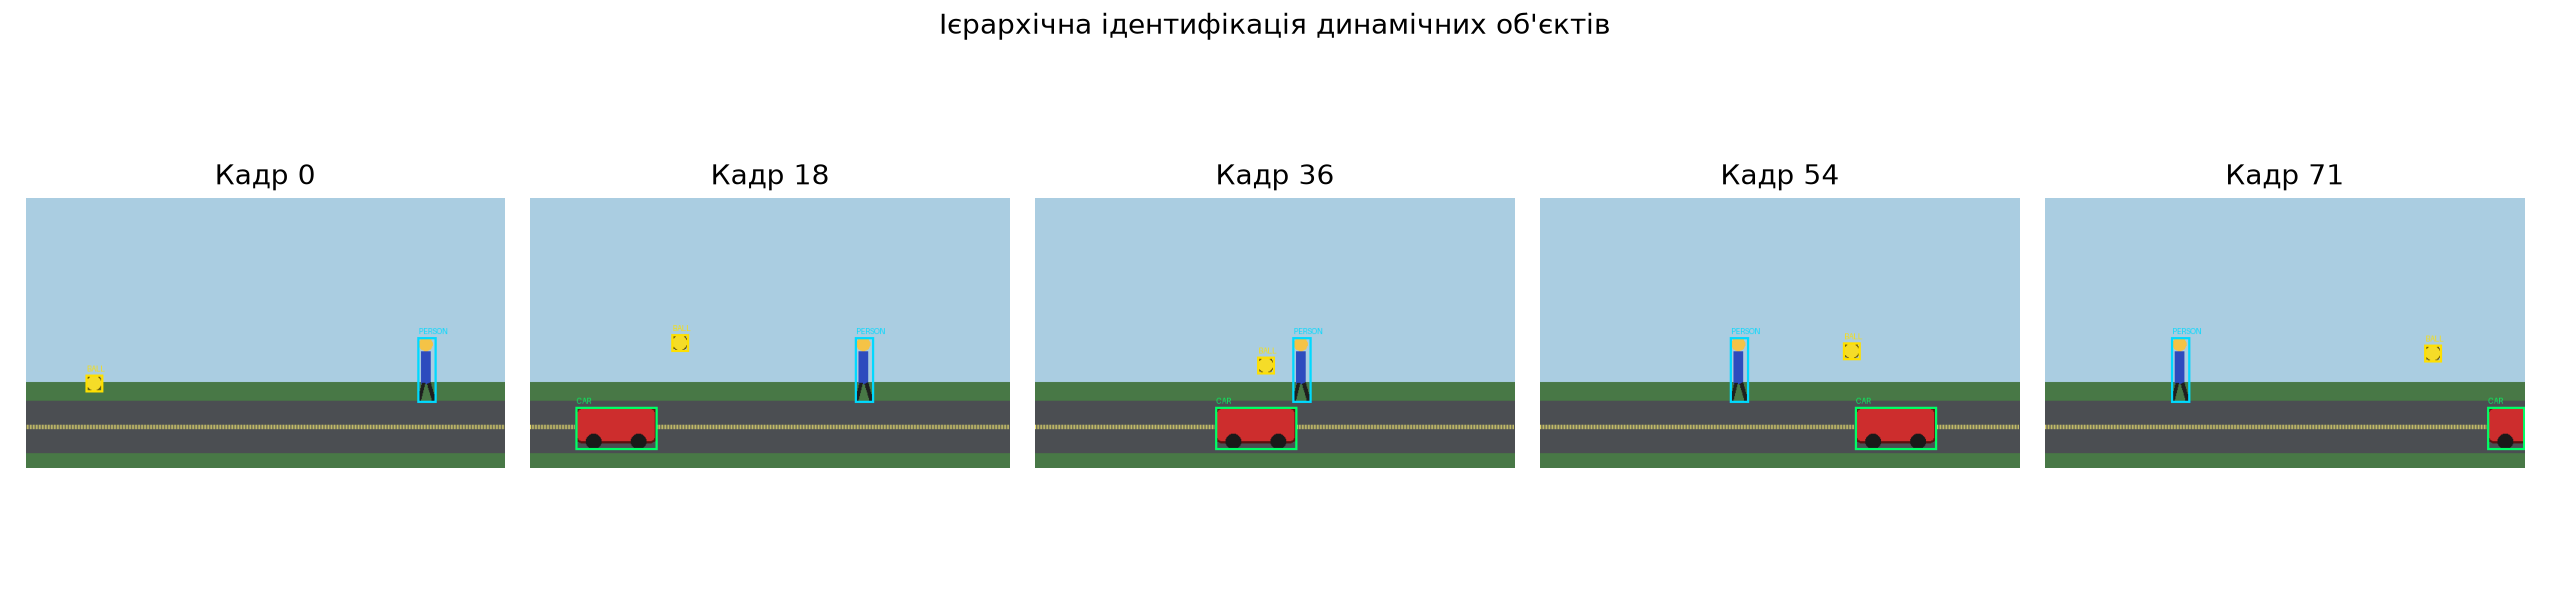
\includegraphics[width=.98\textwidth]{../results/tracking_montage.png}\caption{Ключові кадри ідентифікації динамічних об'єктів}\end{figure}
\begin{table}[H]\centering\caption{Підсумкові показники}
\begin{tabular}{lr}\toprule Показник&Значення\\\midrule Кадрів&72\\Класів&3\\Повнота ідентифікації класів&0,9766\\\bottomrule\end{tabular}
\end{table}
Помилки виникають лише за часткового виходу автомобіля за межі кадру або короткочасного дотику компонентів. Отримане значення 97,66\% підтверджує працездатність ієрархії на контрольному потоці.

\section{Структура проєкту}
\begin{verbatim}
lab6/
|-- src/main.py
|-- results/tracking.gif, tracking_montage.png, detections.csv
|-- requirements.txt
`-- docs/main.tex, main.pdf
\end{verbatim}

\section{Висновки}
Реалізовано повний цикл ідентифікації у відеопотоці: віднімання фону, морфологічну обробку, пошук компонентів, обчислення ознак і послідовну класифікацію. На 72 кадрах повнота склала 97,66\%. Метод не потребує навчальної вибірки й добре пояснюється, але його пороги залежать від масштабу сцени та розташування камери.

\section{Лістинг програми}
\VerbatimInput[fontsize=\small,numbers=left,breaklines=true,frame=single]{../src/main.py}
\end{document}
